\chapter{System Details}


The electroplating system is an unstable system that relies on multiple parameters being within their respective optimal ranges to achieve a desired mode. 
Several tips can help reduce noise and stabilize the system, such as avoiding the use of an oscilloscope with the charger to reduce power line noise. 
Mechanical noise in the pumping machine can be minimized by using a syringe pump tilted with a bubble inside. 
External electrical noise can be picked up by antennas or connections in the circuit. 
And gas pipeline with air into the chamber can be used to stabilize internal humidity and temperature.

The picture in figure \ref{fig:setup_pic} shows the setup used in all this project. Figure \ref{fig:nozzleElectr} shows the nozzle and plate with the charged liquid being electrosprayed in cone jet mode.

\begin{figure}[H]
  \centering
  \resizebox{150mm}{!}{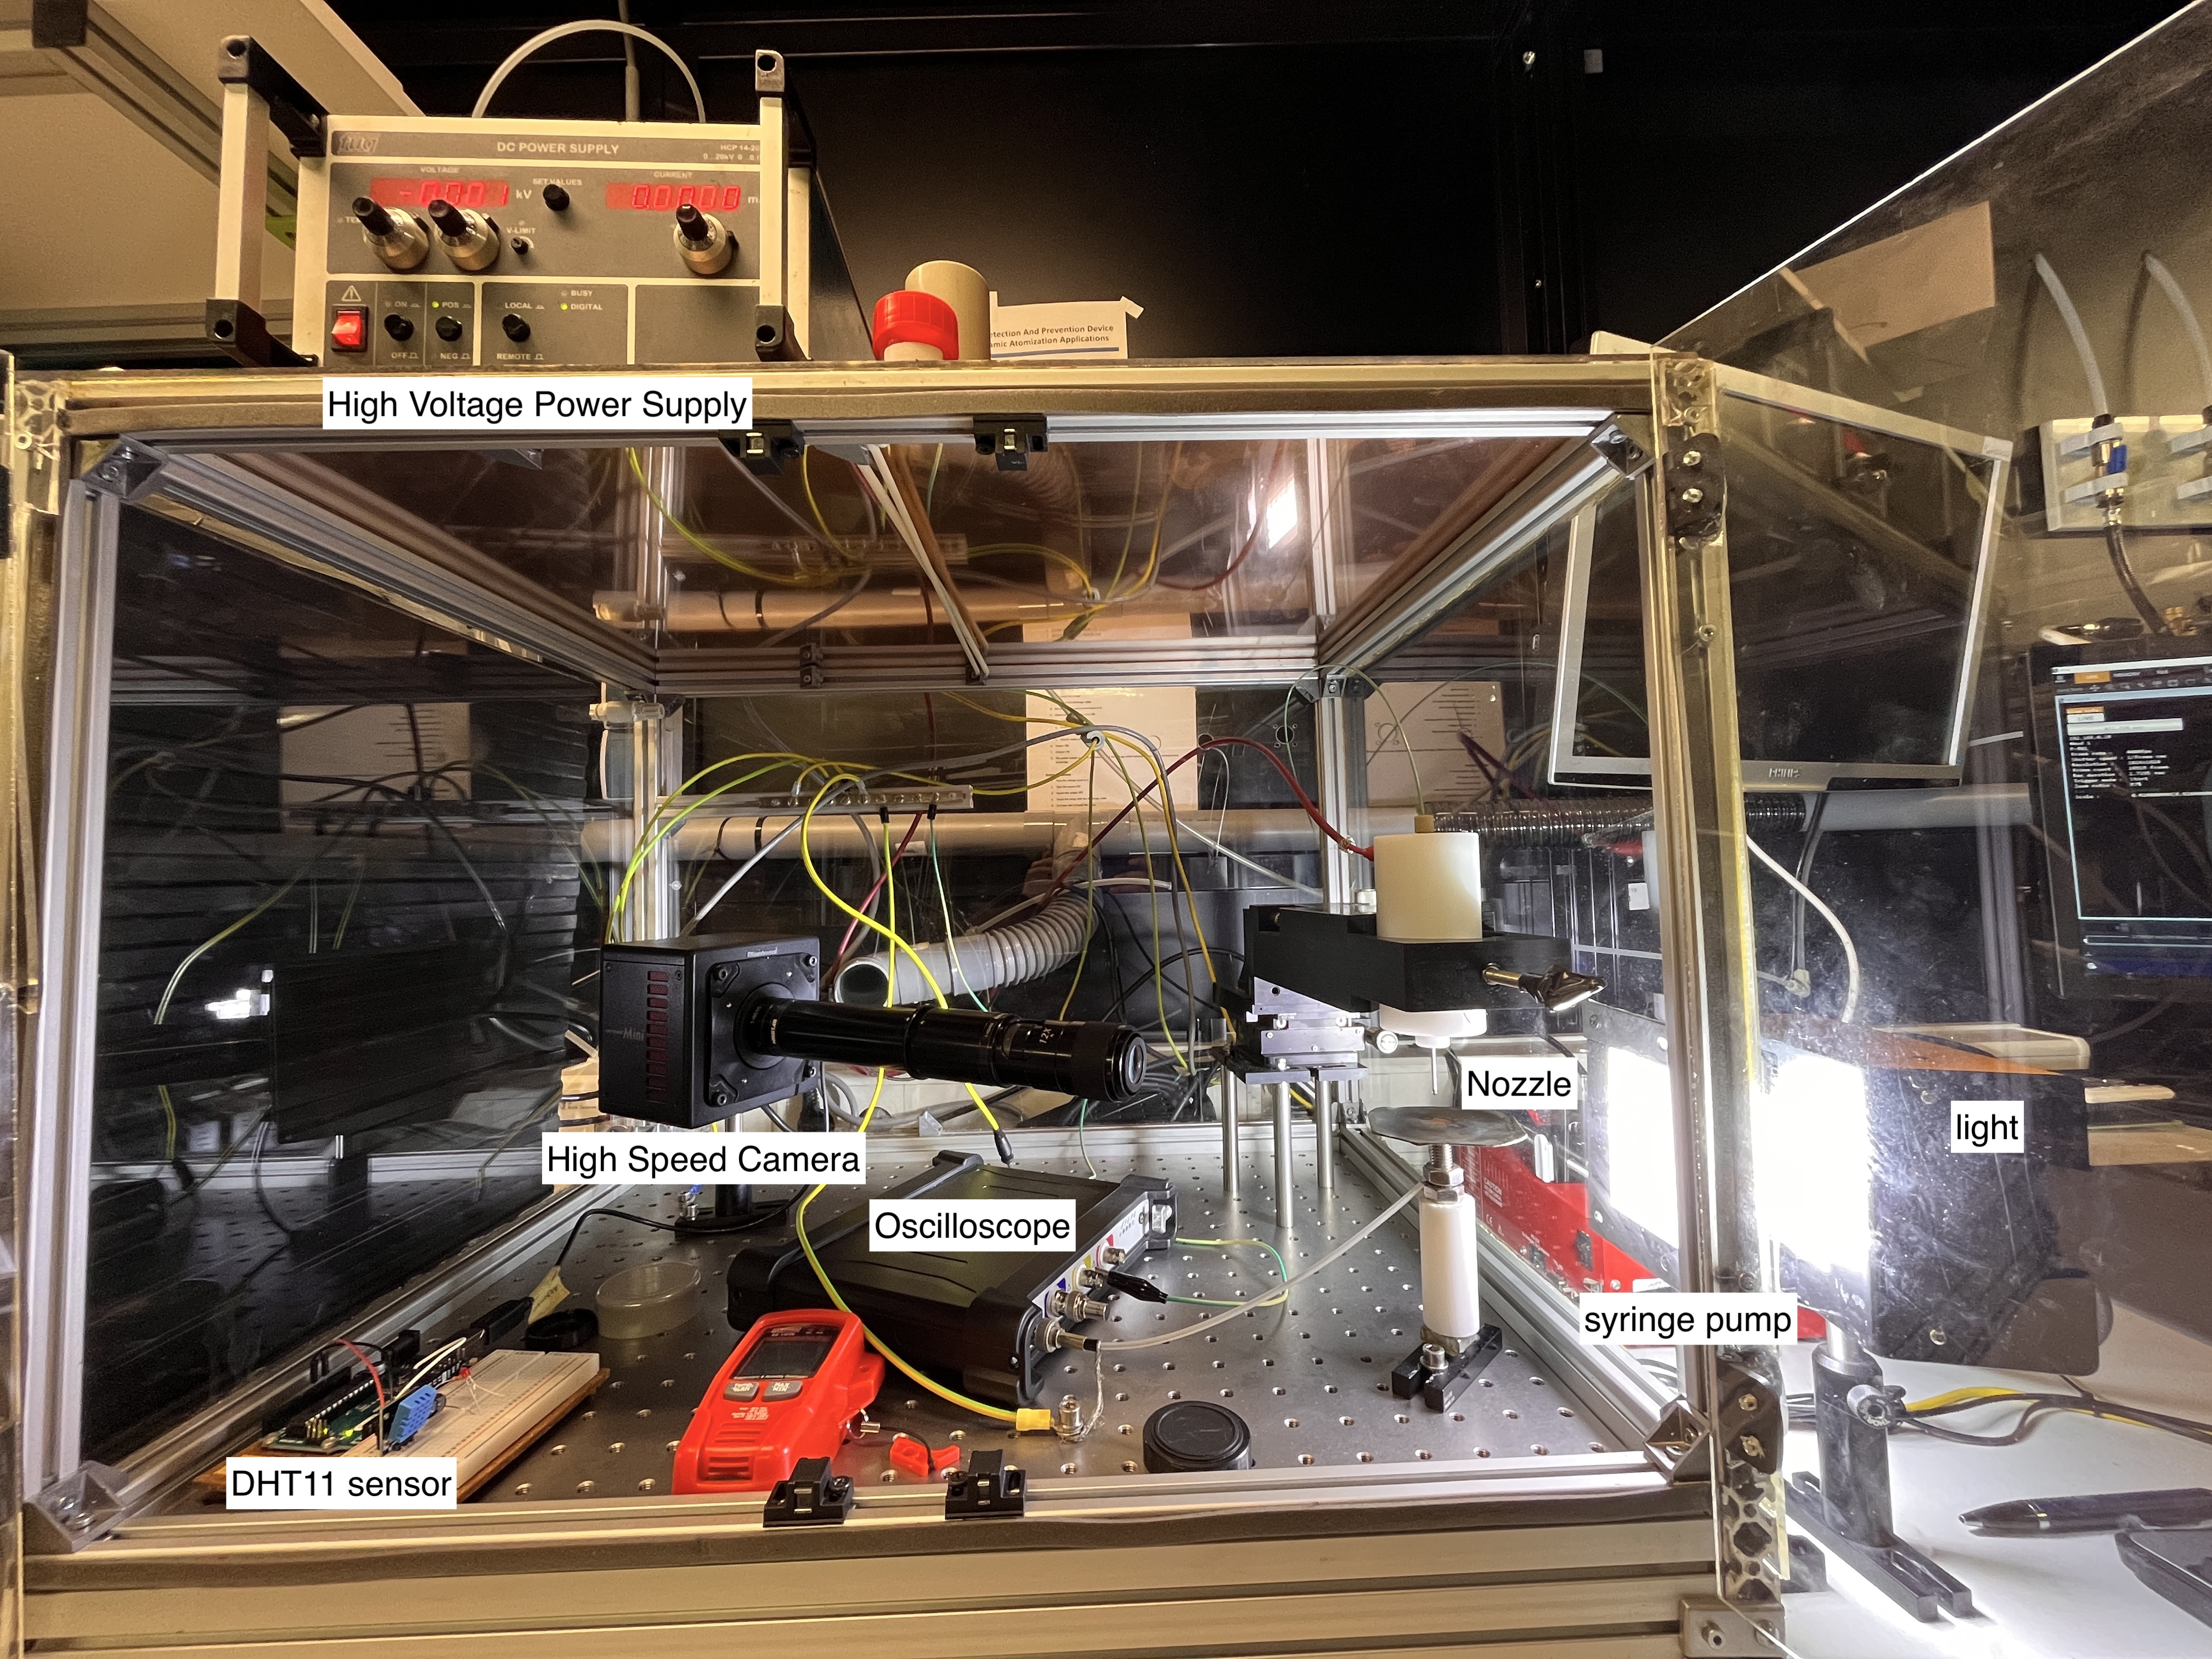
\includegraphics{Figuras/setup_pic.jpg}}
  \caption{EHDA automation system setup used for experiments.}
  \label{fig:setup_pic}
\end{figure}

\begin{figure}[H]
    \centering
    \resizebox{80mm}{!}{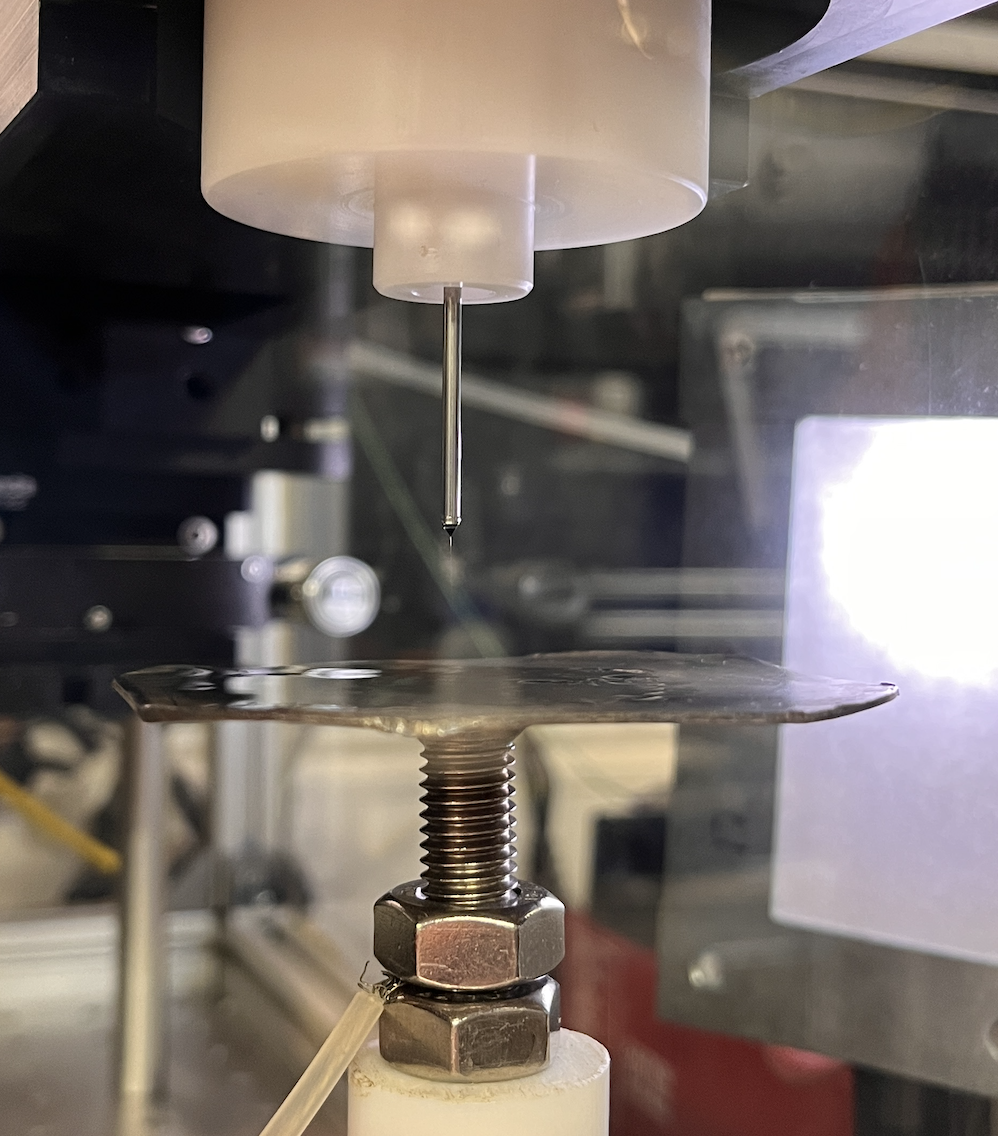
\includegraphics{Figuras/naked_eyes.png}}
    \label{fig:nozzleElectr}
    \caption{EHDA picture of the electrified syringe.}
\end{figure}

